%%%%%%%%%%%%%%%%%%%%%%%%%%%%%%%		CHAP 2		%%%%%%%%%%%%%%%%%%%%%%%%%%%%%%%

\chapter{The ANNIE Experiment}
\label{cha:2}

Final-state neutron abundance from pure neutrino interactions in relation to the energy %
and the direction of final-state muons with respect to the original neutrino %
are currently poorly-known and difficult to measure.
These combined data can be used to better constrain nuclear models of neutrino interaction %
physics and are an essential input to Monte Carlo models, used for calculating %
detection efficiencies, expected background rates, accurate limits, and confidence levels.
The count of neutrons can also be used to reject contamination by atmospheric %
neutrino interactions in proton decay experiments and in a sample of diffuse supernova %
background neutrinos and may also help to statistically address wrong-sign contamination %
in oscillation analyses.
In addition to helping understand fundamental neutrino-interaction physics, tagging events %
by the presence and number of final-state neutrons can provide physics analyses with a better %
handle for signal-background separation and even allow for discrimination between %
different types of neutrino interactions.

\begin{wrapfigure}{L}{0.5\textwidth}
  \centering
  
\includegraphics[scale=.2]{pics/logo_2}
  \caption{Logo of the ANNIE experiment.}
  \label{fig:logo}
\end{wrapfigure}

The \textbf{A}ccelerator \textbf{N}eutrino \textbf{N}eutron \textbf{I}nt\-er\-ac\-tion %
\textbf{E}xperiment (ANNIE) will provide a complementary measurement of neutron yields in %
neutrino-nucleon interactions.
The ANNIE experiment is a prototype neutrino detector currently taking data at the %
Fermi National Accelerator Laboratory (FNAL, Fermilab), in Chicago, USA.
It consists of a small water Cherenkov detector, placed at the former location of %
the SciBooNE experiment~ref[Phys. Rev. D 78 (2008) 112004] and %
deployed on the intense Booster Neutrino Beam (BNB).
An upstream forward Veto and a downstream Muon Range Detector (MRD) are also installed %
in the hall.
The experiment aims to be a test bed for many new technologies, as the gadolinium-doped water %
and the use of early prototype Large Area Picosecond Photodetectors (LAPPDs).
Neutron tagging in Gd-loaded water may play a significant role
in reducing backgrounds from atmospheric neutrinos in next generation 
proton-decay searches using megaton-scale Water Cherenkov detectors, like Hyper-Kamiokande~ref.
Similar techniques might also be useful in the detection of supernova neutrinos. 
Accurate determination of neutron tagging efficiencies will require a 
detailed understanding of the number of neutrons produced by neutrino interactions 
in water as a function of momentum transferred.
To achieve this task, an innovative aspect of the ANNIE design is the use of precision %
timing to localize interaction vertices in the small fiducial volume of the detector.
This experiment will be a first application of these devices demonstrating
their feasibility for Water Cherenkov neutrino detectors.

The experiment is planned to proceed in two stages, spread over five years:
\begin{itemize}
  \item[\bfseries Phase I] a partially-instrumented test-beam run using only Photomultipliers %
    (PMTs) for the purpose of measuring critical neutron backgrounds to the experiment;
  \item[\bfseries Phase II] a longer run with a more fully-instrumented detector %
    where incremental research and development for the LAPPDs and %
    accompanying fast electronics will be fulfilled, as long as the expansion of the %
    photodetector coverage (both LAPPDs and PMTs) required.
\end{itemize}

\emph{Year 1} will focus on the R\&D, particularly on the development of the Data Acquisition %
system, along with the testing in water of the first model of LAPPD. 
Installation of the first LAPPDs and a significant fraction of the additional PMTs, as %
well as the calibration system, will take place in \emph{Year 2}.
Data-taking would commence in \emph{Year 3} and continue through \emph{Year 5}, %
with the physics reach of the detector improving as the fraction of LAPPDs increases over time.
Publication of derived results would occur by the end of \emph{Year 5}.

This thesis is placed at the beginning of \emph{Year 1}, where testing of the Phase I %
experimental setup is tested and R\%D is undertaken.

\section{Neutrino beam}

ANNIE is run on axis from the \emph{Booster Neutrino Beam} (BNB), which deploys %
\np{8.89}~GeV protons accelerated from the Fermilab booster operating at 15~Hz.
The primary beam from the \emph{Linac} uses protons accelerated to 8 GeV kinetic energy %
by the Fermilab booster. 
Selected batches containing approximately \np{5e12} protons are extracted %
and bent toward a beryillium target via dipole magnets.
Each spill is composed of 81 bunches of protons, approximately 6~ns wide each %
and 19~ns apart, for a total spill duration of $\np{1.6}~\mu$s.
Beam proton trajectories and positions are monitored on a pulse-by-pulse basis.
Upstream of the target, the primary proton beam is monitored on a pulse-by-pulse basis %
using four systems: %
two toroids measuring its intensity (protons-per-pulse), beam position monitors %
(BPM) and a multiwire chamber determining the beam width and position, %
and a resistive wall monitor (RWM) measuring both the time and intensity of the beam spills.
A logic signal is also generated by the last device for every intensity peak.
It is employed to trigger the experiment in correspondence of each spill.
The BNB is dealt in detail in the appendix~\ref{app:A}.

\begin{wrapfigure}{R}{0.5\textwidth}
%\begin{figure}[]
  \centering
  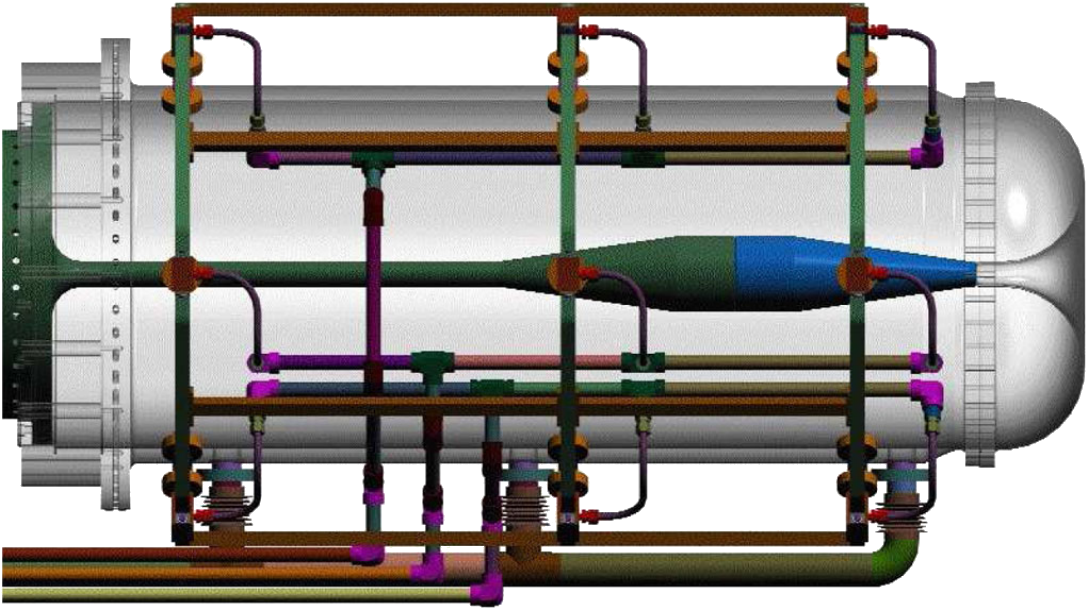
\includegraphics[scale=.2]{pics/bnbhorn}
  \caption{BNB horn system.}
  \label{fig:bnbhorn}
\end{wrapfigure}

Hadronic interactions of the protons with the target material produce a beam of %
secondary mesons, mostly pions and kaons. 
A magnetic focusing horn, shown in Fig.~\ref{fig:bnbhorn}, surrounds the beryllium target, %
bending and sign-selecting the secondary particles emitted along the direction pointing to the hall.
The focusing is produced by the toroidal magnetic field present in the air volume %
between the horn’s two coaxial conductors made of aluminum alloy. 
The beam of focused, secondary mesons emerging from the target/horn region is further collimated, %
via passive shielding, and allowed to decay into neutrinos in a cylindrical decay %
region filled with air at atmospheric pressure, 50~m long and 90~cm in radius. 

The polarity of the horn current flow can be (and has been) switched, in order to %
focus negatively charged mesons, and therefore produce an antineutrino instead of a neutrino beam.
The $\pi^{\pm}$ mesons have a mass of \np{139.6}~MeV and a mean lifetime of \np{2.6e-8}~s.
The primary decay mode of a pion, with a branching fraction of \np{99,9877}\,\%, is a leptonic %
decay into a muon and a muon neutrino:
\begin{align}
  \pi^+ &\rightarrow \mu^+ \, \nu_\mu \\
  \pi^- &\rightarrow \mu^- \, \bar{\nu}_\mu
\end{align}
The second most common decay mode of a pion, with a branching fraction of \np{0.0123}\,\%, %
is also a leptonic decay into an electron and the corresponding electron antineutrino:
\begin{align}
  \pi^+ &\rightarrow e^+ \, \nu_e \\
  \pi^- &\rightarrow e^- \, \bar{\nu}_e
\end{align}

In spite of the considerable differences in the space momentum, the suppression of the %
electronic decay mode with respect to the muonic one is a well known effect, called %
\emph{helicity suppression}: due to the great mass of the muon ($m_\mu = \np{105.658}$~MeV) %
compared to the electron ($m_e = \np{0.510}$~MeV), the helicity-chirality correspondence %
is stronger for the latter.
Given that the $\pi$ mesons are spinless, neutrinos are left-handed, and antineutrinos are %
right-handed, the muonic channel is preferred because of spin and linear momentum preservation.
The suppression of the electronic decay mode with respect to the muonic one is given %
approximately within radiative corrections by the ratio:
\begin{equation}
  R_\pi = \Bigl ( \frac{m_e}{m_\mu} \Bigr )^2 
  \Bigl (\frac{m_\pi^2 - m_e^2}{m_\pi^2 - m_\mu^2} \Bigr )
  = \np{1.283e-4}
\end{equation}

\textcolor{red}{Have to add something about muon decay here.}
A beam absorber located at the end of the decay region stops the hadronic and muonic %
component of the beam, and only an almost pure neutrino beam pointing towards %
the detector remains.

\textcolor{red}{From SciBooNE - charged current etc.}
Neutrino flux predictions are the same produced by the SciBooNE collaboration, obtained via a %
\textsc{geant4}-based beam Monte Carlo simulation.
The same simulation code developed by the MiniBooNE Collaboration is used [24], %
where a realistic description of the geometry and materials present %
in the BNB target hall and decay region is used.
Primary protons are generated according to the expected beam optics properties upstream 
of the target.
The interactions of primary protons with the beryllium target are simulated according %
to state-of-the-art hadron interaction data. 
Of particular importance for this analysis is a $\pi^+$ production in proton-beryllium interactions, %
which uses experimental input from the HARP [25] and BNL E910 [26] experiments. 
Production of secondary protons, neutrons, charged pions, and charged and neutral %
kaons is taken into account, and elastic and quasielastic scattering of protons in the target %
are also simulated.
Particles emanating from the primary proton-beryllium interaction in the target are %
then propagated within the \textsc{geant4} framework, which accounts for all relevant %
physics processes. 
Given the importance of the target (beryillium and alluminum) hadronic reactions, these are %
described by custom models, while other hadronic processes %
and all electromagnetic processes (energy loss, multiple scattering, %
effect of horn magnetic field, etc.) are described according to default \textsc{geatn4} physics lists.

\begin{wrapfigure}{R}{0.5\textwidth}
  \centering
  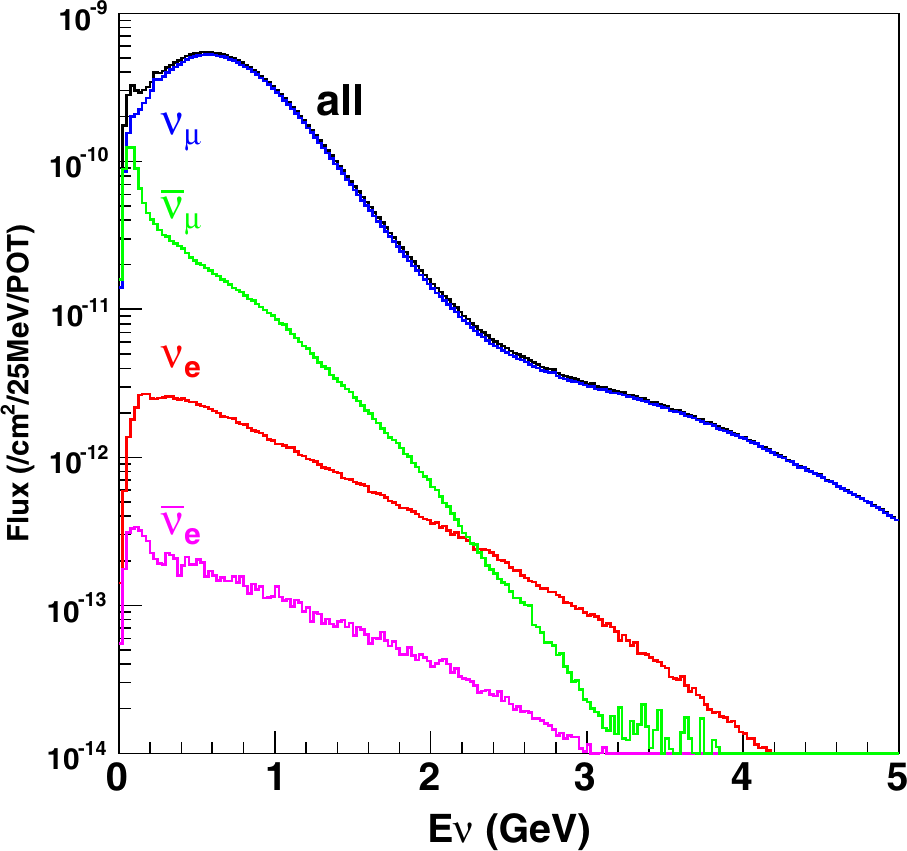
\includegraphics[scale=0.25]{pics/fluxprediction}
  \caption{Neutrino flux predictions from the \textsc{geant4}/FORTRAN simulation.}
  \label{fig:fluxp}
\end{wrapfigure}

A second, FORTRAN-based Monte Carlo code is responsible for generating the neutrino %
kinematics distributions from meson and muon decays, and for obtaining the final neutrino %
fluxes extrapolated to the detector hall with negligible beam Monte Carlo statistical errors. 
Once produced by the simulation, neutrinos are extrapolated along straight lines %
toward the detector and all neutrinos whose traces cross any part of the active volume are %
considered for the flux predictions.
Based on accurate survey data, the distance between the center of the beryllium %
target and the center of the SciBar detector is taken to be \np{99.9}~m, %
with the detector located on beam axis within a tolerance of a few centimeters. 

The neutrino flux prediction at the detector location and as a function %
of neutrino energy is shown in Fig.~\ref{fig:fluxp}.
A total neutrino flux per proton on target of \np{2.2e-8}~cm$^{-2}$ is expected at the %
hall location and in neutrino running mode (positive horn polarity), with %
a mean neutrino energy of \np{0.7}~GeV. 
The flux is dominated by muon neutrinos (93\,\% of total), with small contributions from %
muon antineutrinos (6.4\,\%), and electron neutrinos and antineutrinos (0.6\,\% in total). 
For the neutrino flux predictions, no information from BNB %
(SciBooNE or MiniBooNE) neutrino data was used as experimental input.

\section{The Hall}

The experiment is set up in the former location of the SciBooNE experiment~refagain?, %
8~m below the surface and the 100~m from the BNBtarget.
Already exisiting instrumentation in the hall is borrowed by the ANNIE experiment.

\subsection{Water tank}
\label{2.2}
\textcolor{red}{tank = PMTs, water, future LAPPDs and Gd (NCV). Very messy now}

\begin{wrapfigure}{R}{0.5\textwidth}
  \centering
  \includegraphics[scale=0.25]{pics/ANNIEreduced}
  \caption{Schematic of the experimental hall.}
  \label{fig:anniehall}
\end{wrapfigure}

The main component of the experiment is the water tank, installed in the SciBooNE hall %
at Fermilab.
Incom Inc, the company selected to commercialize the LAPPD photodetectors, has provided a
quote to the ANNIE collaboration committing to produce 20 detectors
This is already price-competitive per unit area with equivalent
technologies offering similar capabilities (a single LAPPD covers 16 times the area of a 10k 2”
Photonis Planacon MCP-PMT and 64 times that of an 8k Hamamatsu 1 inch tube).
These early LAPPDs will be produced in small batches over a period of several years, %
with the first two LAPPDs arriving no later than September 2016 and 5-8 more tiles in September 2017.
Specifications of the LAPPDs are derived from prior tests: time resolutions below 100 psec, %
spatial resolutions below 1~cm, and gains above 1x10 7 [21], as well as 20\,\% quantum %
efficiency photocathodes and good gain uniformity [32].
The LAPPD purchase by the ANNIE collaboration represents a technology investment that will %
pay out past its experimental lifecycle.
Their use in ANNIE provides an essential proof-of-principle %
demonstration of the technology and LAPPDs purchased through ISU can be made available for %
future HEP efforts after ANNIE.
Application-specific detector development work necessary to deploy LAPPDs for use %
in water is also required.
The devices need to be characterized and—along with their high voltage connections %
and front-end readout boards—must be mounted and placed in the water volume.%
Water submersion tests (including tests using the full ANNIE water volume) will proceed %
first using several 6~cm photosensors provided by ANL, built using a similar design and %
process to the Incom LAPPDs.
14ANL will also design and provide an 8” x 8” structure on which to mount the 6~cm tiles, %
compatible with the waterproof housing for full-size detectors.
The additional development of electronics to read out the LAPPDs and its impact on the %
overall DAQ system is described in Sec 4.7.
One or more publications on the novel instrumentation of ANNIE are planned.
In order to guarantee physics results from this effort independently of the status of LAPPD %
production, an alternative choice for light detectors will be developed in parallel.
The optimal choice at this stage would appear to be the Hamamatsu H11934-200 ultra %
bialkali 1-inch PMTs.
With a quantum efficiency of 43\,\%, comparable photon collection efficiencies to %
LAPPDs can be achieved with less spatial coverage.
The combination of 270 psec time resolutions and fine granularity of these detectors %
provides capabilities comparable to those discussed in Sec 3.4 (see Fig 6).
A quote for 600 of these tubes has been obtained from Hamamatsu and is comparable in cost %
with the equivalent area x coverage scenario proposed with LAPPDs.
It would rely on the same electronics, and mixed 1-inch and LAPPD scenarios are also possible.
The group at Lawrence Berkeley National Laboratory (LBNL), led by PI Orebi Gann, %
is already working with these tubes in a bench-top scale water-based liquid %
scintillator setup aimed at demonstrating ring imaging for high-energy events in this target medium, %
leveraging funding by the LBNL LDRD program.

Photodetection in ANNIE Run I will be provided by of 60 8 Hamamatsu PMTs, from a stock of %
Super-K spares

\textcolor{red}{Improve Gd section.}
Gadolinium in water (NCV)
EDGAS and other experiments.
The Super-Kamiokande (SK) [1] is the largest light water Cherenkov detector %
that has been successfully observing solar, atmospheric and accelerator neutrinos.
Recently the addition of 0.2\,\% of a water soluble gadolinium (Gd) compound to SK %
has been proposed [2].
This modification can greatly improve the detection sensitivity of anti-electron neutrinos.
The inverse beta interaction in the water, emits a positron and a neutron.
The positron, radiating Cherenkov photons, is immediately detected.
The neutron is quickly thermalized in the water, and is then captured by Gd with a %
probability of 90\,\%.
Upon capturing a neutron the Gd emits 3-4 gamma rays having a total energy of %
about 8 MeV.
The time and spatial correlation of the positron and neutron capture events (20 us and 4 cm) %
can significantly reduce the backgrounds, and hence enhance the nu e signal events.

\subsection{Photodetectors+LAPPDs}
\label{2.2.1}
Photomultiplier tubes
As noted earlier, ANNIE Phase II will achieve the necessary coverage to detected neutron capture
in Gd-loaded water using by: (1) utilizing twenty in-hand 11-inch L PMTs (refurbished %
proto-types developed under R\&D grants from the NSF and DNN), (2) purchasing 50 new HQE 10-inch %
Hamamatsu PMTs (45+5 spares), and (3) re-using the 8-inch Hamamatsu PMTs refurbished by %
UC Irvine for ANNIE Phase I.
We request funds to purchase the HQE 10-inch PMTs, but with a reserve option to purchase %
140 new 8-inch normal QE PMTs (the higher-cost, higher-channel-density option).
More detailed simulations will enable a final decision by the collaboration before %
procurement of the conventional PMT system.
Calibration, testing and installation of these PMTs will be carried out by UC Davies and/or UC Irvine.

List of pmts employed??

Talk about LAPPDs

\subsection[MRD and VETO]{Muon Range Detector+Veto}
\label{2.3}
\textcolor{red}{mostly ok, I guess I have every information.}

A Forward Anti-Coincidence Counter (FACC) consisting of two layers of overlapping muon %
paddles detects charged particles produced in the dirt upstream of the hall.
This allows the rejection of events in the tank unrelated to the beam.

An iron-scintillator sandwich muon range detector (MRD), already in the experimental hall, %
will be used to range out and fit the direction of daughter muons from neutrino interactions %
in the water target.
Neutrino interactions in the water target will produce light with no signal in the FACC and those
that are muon neutrino charged current will likely produce a muon going through the MRD.

The role of the Muon Range Detector is to confine the muons produced in charge-current %
quasi-elastic (CCQE) interactions, which is the dominant process in SciBooNE.
By confining the muon its energy can be reconstructed thus giving a handle on the neutrino %
energy.
The MRD consists of 13 alternating horizontal and vertical scintillator planes, %
each separated by a 5~cm iron sheet.
This results in 60~cm of absorber equivalent to %
stopping a 1 GeV muon.
The first plane is directly downstream of the EC allowing for %
better track matching and energy reconstruction of pai0 decay photons that escape the EC. 
Three planes are required to be hit for a track to be reconstructed in the MRD, equivalent %
to approximately a 180~MeV muon.
The total mass of the detector is 60 tonnes, of which %
approximately 48 tonnes is absorber.
Planes can be moved forward or backward via the use %
of winches attached to the side of the support frame.
There are 362 channels in total; 182 horizontal, 180 vertical.
Each channel is 20 cm wide and either 155 cm (horizontal) or 138 cm (vertical) long.
Planes have active areas of 310per260 cm 2 (horizontal) and 300per276 cm 2 (vertical).
Of these 362 channels 5 different photomultiplier tubes (PMTs) are used.
The horizontal planes consist of 14 stage EMI 9954KB PMTs from the KTeV experiment, %
as well as EMI 9839b and 9939b PMTs.
The vertical planes consist of 10 stage Hamamatsu 2154-05 PMTs from %
the NuTeV experiment and RCA 6392A PMTs.
The electronics consist of LeCroy 4300B ADCs, LeCroy 3377 %
TDCs and the LeCroy 1440 high voltage system.

ANNIE makes use of an existing Muon Range Detector (MRD) that remains mostly intact in the %
experimental hall.
The MRD is a steel and plastic scintillator sandwich detector, designed to range %
GeV-scale muons and provide directional information.
The electronics and high voltage %
(both for the MRD and photosensors in the water volume) will be provided by Fermilab PREP %
for the duration of the experiment.
Several layers of muon paddles and PMTs are absent; Fermilab has agreed to provide %
materials and instructional support to the ANNIE collaboration to replace the %
missing paddles.

\begin{wrapfigure}{L}{0.5\textwidth}
  \centering
  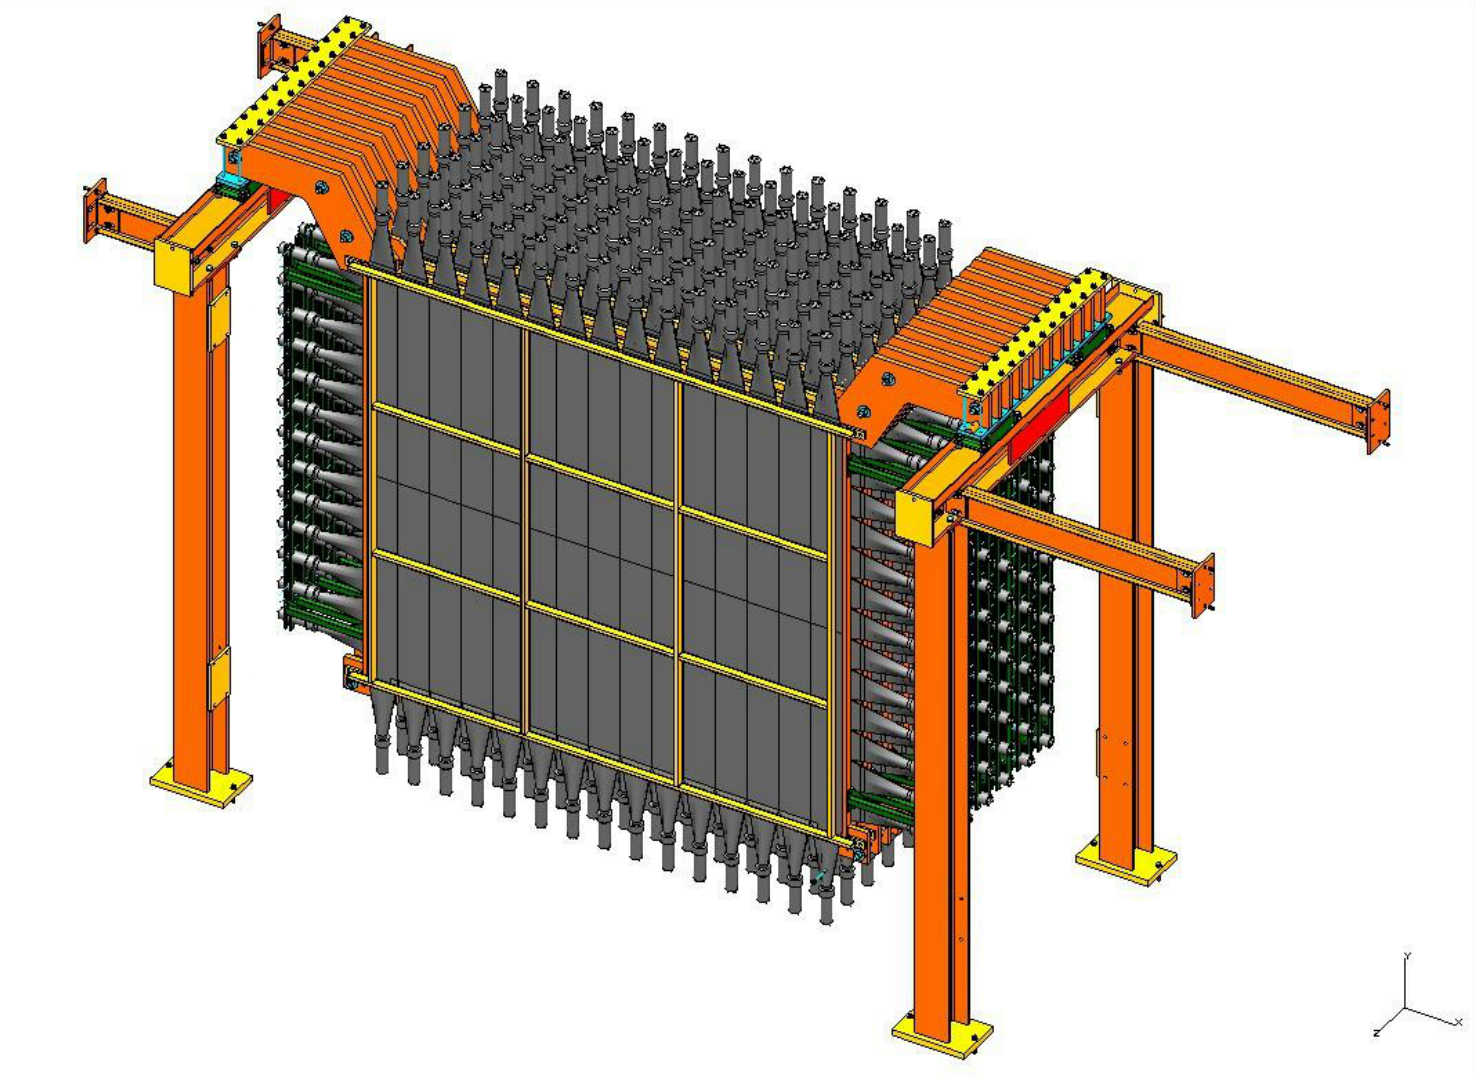
\includegraphics[scale=.15]{pics/pag23Nakajimathesis}
  \caption{Drawing of the MRD.}
  \label{fig:mrd}
\end{wrapfigure}


A fraction of the MRD will be made operational for Phase I of ANNIE in early fall.
Refurbishment activities by UC Davies will be scheduled after this phase is completed taking %
so that the detector system is fully operational in time for ANNIE first physics runs.
ANNIE will rely on a Forward Anti-Coincidence Counter (FACC) consisting of 2 layers %
of overlapping muon paddles to reject charged particles produced in dirt, upstream of the hall.
Fermilab provided a stock of 60 muon paddles taken from the CDF experiment, from which a subset %
of 26 paddles were systematically tested and selected.
These paddles have already been attached to the wall by students from UC Davis with %
the help of Fermilab technicians, using standard 80/20 aluminum extrusions and brackets, %
arranged in two staggered layers of 13 paddles each.

\begin{figure}[]
  \centering
  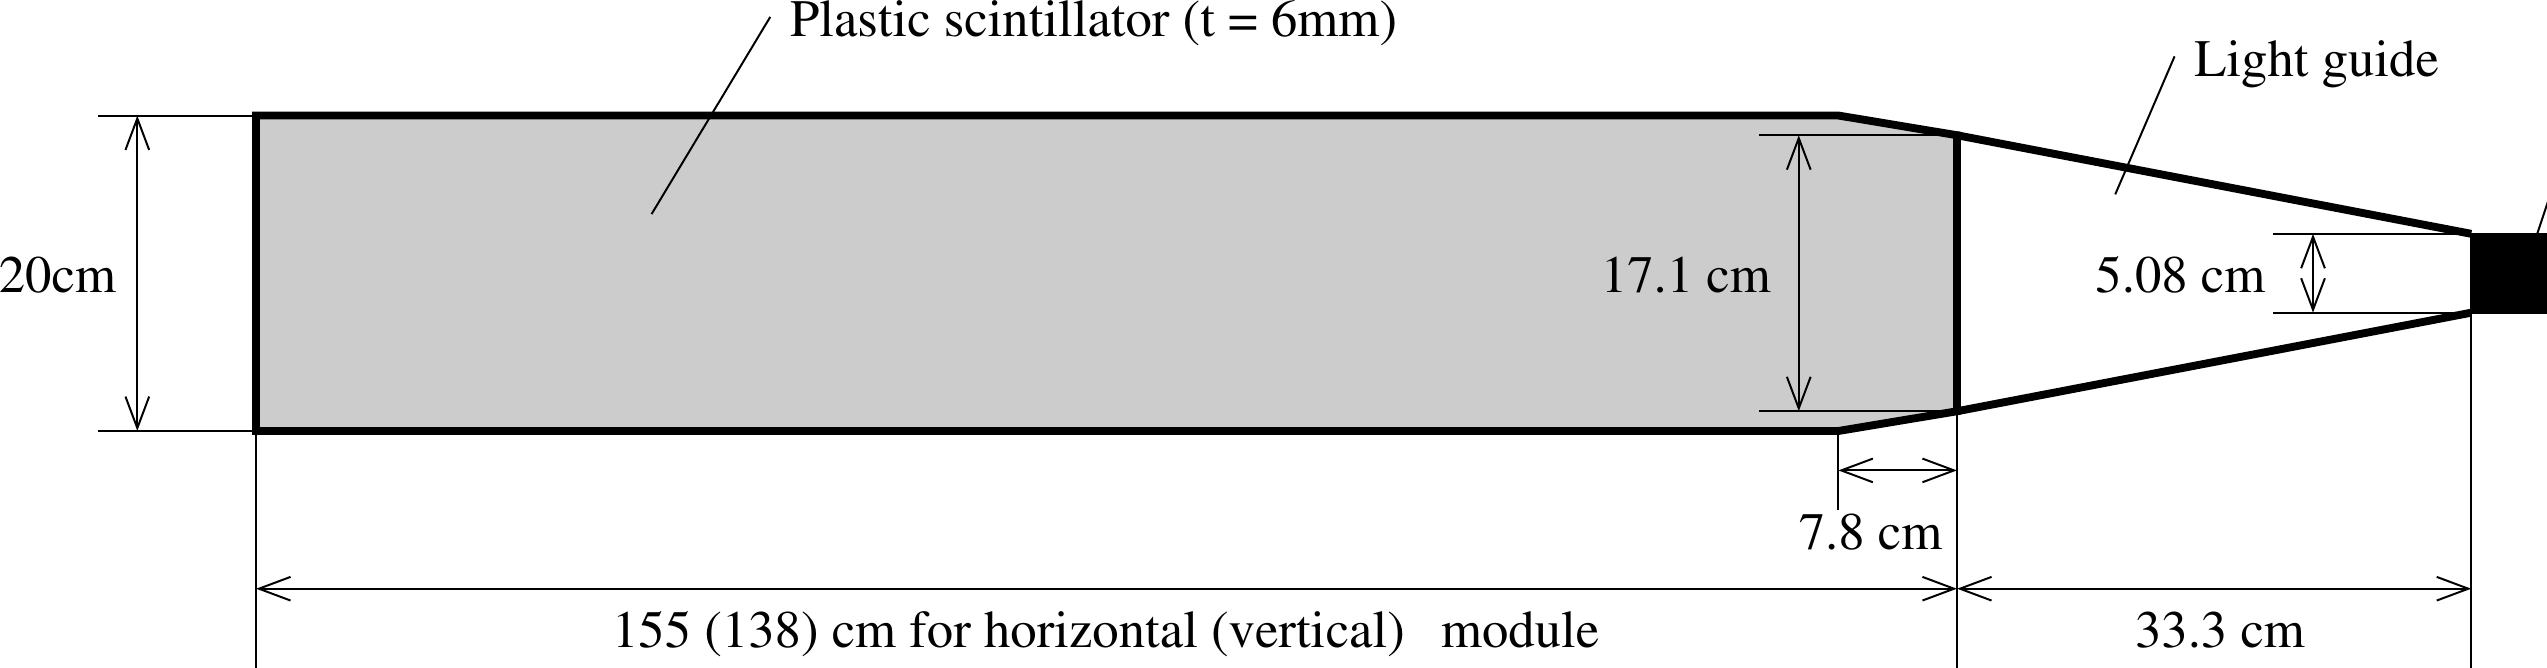
\includegraphics[scale=0.20]{pics/pag24Nakajimathesis}
  \caption{Paddle used for the MRD.}
  \label{fig:paddle}
\end{figure}

\section{Expected events}
\label{2.4}
\textcolor{red}{Odd section.}
A beam event should produce a muon in the tank, so the Veto shouldn't fire, %
some Cherenkov light could be captured by the PMTs and a clear signal is found in the MRD.
